\documentclass[runningheads,a4paper]{llncs}

%%% Some recommended packages.
%\usepackage{booktabs}   %% For formal tables:
%                        %% http://ctan.org/pkg/booktabs
%\usepackage{subcaption} %% For complex figures with subfigures/subcaptions
%                        %% http://ctan.org/pkg/subcaption

% Packages usually used by soton
	% Package for input encoding
	\usepackage[utf8]{inputenc}
	
	%\usepackage[T1]{fontenc}
	%\usepackage{lmodern}
	
	% Package for multilingual support, loaded with English support.
	\usepackage[english]{babel}
	
	% Package for fancy quotations
	\usepackage[autostyle]{csquotes}
	
	% Package for URLs
	\usepackage{url}
	
	\usepackage{colourSoton}
	
	% Package for hyper-references
	\usepackage{hyperref}
	\hypersetup{
		colorlinks=true,
		citecolor=red,
		linkcolor=blue,
		urlcolor=cyan,
	}
	
	% Package for graphics
	\usepackage{graphicx}
	\graphicspath{ {img/} }
	
\usepackage[colorinlistoftodos]{todonotes}

% Package for change tracking
	% \usepackage[disabled]{chgtrk}
	\usepackage{chgtrk}
	\newCTcontributor{Colin}
	\newCTcontributor{Son}
	\newCTcontributor{Karla}
	% \newCTcontributor{Michael}
	
	% Package for abbreviation
	\usepackage{abbrev-scxml2020}
	
	% Package for standalone source code
	\usepackage{standalone}
	
	% Package for requirements document
%	\usepackage[compact]{reqdoc}
	
	% Package for TikZ pictures
	\usepackage{tikz}
	\usetikzlibrary{positioning}
	\usetikzlibrary{shapes}
	
	% Custom pgf pictures
%	\usepackage{pgf-picture}
	
	\usepackage{wrapfig}
	
	% Package for listing Event-B code
	\usepackage[colour]{lstEventB}

	\newtheorem{assumption}{Assumption}
% For floating listings
\usepackage{float}
\newfloat{lstfloat}{htbp}{lop}
\floatname{lstfloat}{Listing}
\def\lstfloatautorefname{Listing} % needed for hyperref/auroref
	
	%package for envelope
	\usepackage{bbding}
% end of packages used by soton

\begin{document}

% first the title is needed
% \title{Refinement of Reactive Systems} 
\title{Formal verification and validation of run-to-completion style state-charts using Event-B}

% a short form should be given in case it is too long for the running head
 \titlerunning{Formal V\&V of State-charts} 

% the name(s) of the author(s) follow(s) next
%
% NB: Chinese authors should write their first names(s) in front of
% their surnames. This ensures that the names appear correctly in
% the running heads and the author index.
%
\author{ 
K. Morris \inst{1} 
\and C. Snook \inst{2}%\textsuperscript{https://orcid.org/0000-0002-0210-0983} 
\and T.S. Hoang \inst{2}
\and \\G. Hulette \inst{1}
\and R. Armstrong \inst{1}
\and M. Butler \inst{2} 
}

\authorrunning{Morris, Snook, Hoang et al.}
%% (feature abused for this document to repeat the title also on left hand pages)

%
% the affiliations are given next; don't give your e-mail address
% unless you accept that it will be published
\institute{
	Sandia National Laboratories, 
	7011 East Avenue Livermore, California 94550, USA\\
	\email{\{knmorri\footnote{Corresponding author, ORCID iD: https://orcid.org/0000-0002-0146-3176, telephone: +1(925) 294-3287},rob,ghulett\}@sandia.gov}
	\and
	ECS, University of Southampton,
	Southampton SO17 1BJ, United Kingdom\\
	\email{\{cfs,t.s.hoang,mjb\}@soton.ac.uk}\\
}

%% \maketitle
%% Note: \maketitle command must come after title commands, author
%% commands, abstract environment, Computing Classification System
%% environment and commands, and keywords command.
\maketitle
% \SonComment{I changed the address for University of Southampton}

% !TEX root = ../SCXMLREF.tex
\begin{abstract}

State-chart modelling notations, such as State Chart eXtensible Markup Language (SCXML), with so-called `run to completion' semantics and simulation tools for validation, are popular with engineers for designing machines. However, they do not support refinement and they lack formal verification methods and tools. Properties concerning the synchronisation between different parts of a machine may be difficult to verify for all scenarios.  Event-B, on the other hand, is based on refinement from an initial abstraction and is designed to make formal verification by automatic theorem provers feasible, obviating the need for instantiation and testing. We would like to combine the best of both approaches by incorporating a notion of refinement, similar to that of Event-B, into SCXML and leveraging Event-B's tool support for proof. We describe some the pitfalls in translating 'run to completion' models to Event-B refinements, and suggest a solution and propose extensions to the SCXML syntax to describe refinements. We illustrate the approach using our prototype translation tools and show by example, how a synchronisation property between parallel state-charts can be automatically proven at an incomplete refinement level by translation into Event-B. 

\keywords SCXML, State-charts, Event-B, iUML-B, refinement
\end{abstract}

%%% Local Variables: 
%%% mode: latex
%%% TeX-master: "RailGround"
%%% End: 

% !TEX root = ../main.tex

Possible outline:
\begin{itemize}
\item Motivation
\item Background and Previous Work
\item Description of Sample Application
\item Statechart Refinements
\item Verification of Safety Properties 
\item Results
\item Conclusion 
\end{itemize}

\section{Introduction}

Text for paper
% \section{Introduction}
% Text of paper \ldots
% !TEX root = ../main.tex

%\section{Related Work}
%\label{sec:relatedWork}

The work we will present here includes three refinement rules.
\begin{enumerate}
\item  \emph{Rule A:} Guard conditions on a transition can be strengthened (but not weakened); 
this can be done by adding textual guards to the transition, or
changing the source of the transition to a nested state.
\item \emph{Rule B:} Transitions can have additional actions, provided they do not
  modify variables appearing in the abstraction; this can be 
  accomplished by adding textual action to the transition 
  or by changing the target to nested state.
\item \emph{Rule C:} A state-chart can be embedded within a state of another
  state-chart -- sometimes called hierarchical composition or
  hierarchical refinement.
\end{enumerate}
Via the translation explained in Section~\ref{sec:translation}, these
rules rely on the usual \EventB proof obligations to ensure that they
do indeed yield refinements in the \EventB semantics.  If an \EventB
model |B| can be shown (via the construction rules of the \EventB
language as well as the proof obligations) to refine another \EventB
model |A|, then we know that every behavior of |B| is also a behavior
of |A|. This definition yields a useful principle of preservation of
safety -- if we can show that a bad thing never happens in |A|, then
we can add detail via refinements in |B|, knowing that the bad thing
will continue to never happen in |B|. That is, \EventB refinements
preserve safety properties in the sense adopted by Lamport
~\cite{lamport1977proving}. This makes refinement a useful technique
in developing safety-critical systems: one can analyze a simpler
abstract model for critical safety properties and then add detail to
the model via refinements, secure in the knowledge that the safety
properties will be preserved. While \EventB refinements have also been
shown to preserve some liveness properties under certain
conditions~\cite{hoang2016ltl}, there are not yet efficient supporting
tools for the technique. Instead, we can express the property in \LTL
and use the \PROB\footnote{ProB is an animator, constraint solver and
  model checker for the B-Method. https://www3.hhu.de/stups/prob}
model checker to verify it, as we have shown in previous
work~\cite{detect2020}.  In this paper, we outline a proof of liveness
properties that relies on reasoning about deadlock-freeness and event
convergence.


% Although the autonomous drone example in this paper is based on the
% example described in~\cite{Syriani_2019}, the definition of refinement
% used in that work is quite different from our own. This forces some
% differences in our refinement rules and consequently the way the
% example is developed.  In~\cite{Syriani_2019} ``refinement'' is a
% transformation of the model which preserves reachability of a state
% with respect to sequences of inputs. However, this also allows the
% possibility of introducing new behaviors in the concrete model that
% the abstraction does not exhibit (more details are in
% Section~\ref{sec:descr-sample-appl}). While this notion of refinement
% seems useful in certain contexts, unlike refinement in \EventB it does
% not guarantee preservation of safety properties. Therefore it should
% be considered less suited to development of safety-critical systems.

%%% Local Variables:
%%% mode: latex
%%% TeX-master: "../main"
%%% End:
% !TEX root = ../SCXMLREF.tex

\section{Background}
\label{sec:background}

% !TEX root = ../main.tex

\subsection{SCXML}
\label{sec:scxml}

\SCXML is a modelling language based on Harel state-charts with facilities for adding data elements that are modified by transition actions and used in conditions for their firing~\cite{scxmlwebsite}. 
\SCXML follows a `run to completion' semantics, where trigger events\footnote{In \SCXML the triggers are called `events', however, we refer to them as `triggers' to avoid confusion with \EventB} may be needed to enable transitions.
Trigger events are queued when they are raised, and then one is de-queued and consumed by firing all the transitions that it enables, followed by firing the un-triggered transitions that become enabled due to the change of state caused by the initial transition firing.
This is repeated until no transitions are enabled, and then the next trigger is de-queued and consumed.
Note that the enabledness of transitions is calculated batch-wise at each step, not after each and every transition.
Hence the set of parallel transitions that are enabled by a trigger is calculated and then only those are fired, irrespective of whether firing one may disable or enable another.
Similarly, the set of parallel untriggered transitions to be fired is calculated at each iteration before any is fired.
There are two kinds of triggers: internal triggers are raised by transitions and external triggers are raised by the environment (non-deterministicly for the purpose of our analysis). 
An external trigger may only be consumed when the internal trigger queue has been emptied.
We chose \SCXML as our source language because it is relatively simple compared to some run to completion modelling languages yet has a well defined action language and simulation tool support.

\ColinInlineComment{I have added the pseudocode back in because i like it (we removed it for space for detect) }

Listing~\ref{lst:scxml-r2c} shows a pseudocode representation of the run to completion semantics as defined within the latest W3C recommendation document~\cite{scxmlwebsite}. Here IQ and EQ are the triggers present in the internal and external queues respectively. We adopt the commonly used terminology where a single transition is called a \emph{micro-step} and a complete run (between de-queueing external triggers) is referred to as a \emph{macro-step}.

 \begin{lstlisting}[caption=Pseudocode for 'run to completion',label={lst:scxml-r2c}, frame=single]
 while running:
 	while completion = false
 		if untriggered_enabled
 			execute(untriggered())
 		elseif IQ /= {}
 			execute(internal(IQ.dequeue)) 
 		else
 			completion = true
 		endif
 	endwhile
 	if EQ /= {}
 		execute(EQ.dequeue) 
 		completion = false
 	endif
 endwhile 
 \end{lstlisting}



%%% Local Variables: 
%%% mode: latex
%%% TeX-master: "../main.tex"
%%% End: 

% !TEX root = ../SCXMLREF.tex

\subsection{Event-B}
\label{sec:eventb}

\eventB~\cite{abrial10:_model_event_b} is a formal method for system
development.  Main features of \eventB include the use of
\emph{refinement} to introduce system details gradually into the
formal model.  An \eventB model contains two parts: \emph{contexts} and \emph{machines}. Contexts contain \emph{carrier sets}, \emph{constants}, and \emph{axioms} constraining the carrier sets and constants.  Machines contain \emph{variables} \Bv, \emph{invariants} $I(\Bv)$ constraining the variables, and \emph{events}. An event comprises a guard denoting its enabled-condition and an action describing how the variables are modified when the event is executed.  In general, an event \Be has the following form, where \Bt are the event parameters, $G(\Bt, \Bv)$ is the guard of the event, and $S(\Bt, \Bv)$ is the action of the event.
\begin{align}
& \inlineevent{\Be}{}{\Bt}{G(\Bt,\Bv)}{}{S(\Bt,\Bv)}
\end{align}
In the case where the event has no parameters, we use the following form
\begin{align}
& \inlineevent{\Be}{}{}{G(\Bv)}{}{S(\Bv)}~,
\end{align}
and when the event has no parameters and guard, we use
\begin{align}
& \inlineevent{\Be}{}{}{}{}{S(\Bv)}~.
\end{align}
The action of an event comprises of one or more assignments, each of them has one of the following forms.
\begin{align}
& \Bv \bcmeq E(\Bt, \Bv) \label{eq:bcmeq}\\
& \Bv \bcmin E(\Bt, \Bv) \label{eq:bcmin}\\
& \Bv \bcmsuch P(\Bt, \Bv) \label{eq:bcmsuch}
\end{align}
Assignments of the form \eqref{eq:bcmeq} are deterministic, assign value of expression $E(\Bt, \Bv)$ to \Bv.  Assignments of the forms \eqref{eq:bcmin} and \eqref{eq:bcmsuch} are non-deterministic. \eqref{eq:bcmin} assigns any value from the set $E(\Bt,\Bv)$ to \Bv, while \eqref{eq:bcmsuch} assigns any value satisified predicate $P(\Bt,\Bv)$ to \Bv.
Note that invariants $I(\Bv)$ are inductive, i.e., they must be \emph{maintained} by all events. This is more strict than general safety properties which hold for all reachable states of the \EventB machine.  This is also the difference between verifying the consistency of \EventB machines using theorem proving and model checking (e.g., \PROB) techniques: model checkers explore all reachable states of the system while interpreting the invariants as safety properties.

A machine in \eventB corresponds to a transition system
where \emph{variables} represent the states and \emph{events} specify
the transitions.    More information about \eventB can be found in~\cite{hoang13:_introd_event_b_model_method}.  \eventB is supported by the
\Rodin~\cite{abrial10:_rodin}, an extensible toolkit which includes
facilities for modelling, verifying the consistency of models
using theorem proving and model checking techniques, and validating
models with simulation-based approaches.

In Event-B the run to completion pseudocode of Listing~\ref{lst:scxml-r2c} could be represented (somewhat abstractly) as

\begin{Bcode}
	$%
	\event{FireUntriggered}{}{}{UC=FALSE}{}{execute(untriggered())}
	\event{FireInternallyTriggered}{}{}{UC=TRUE\\IQ\neq\emptyset}{}{execute(IQ.dequeue)\\UC:=FALSE}
	\event{FireExternallyTriggered}{}{}{UC=TRUE\\IQ=\emptyset\\EQ\neq\emptyset}{}{execute(EQ.dequeue)\\UC:=FALSE}
	$
%	\Bvspace[2ex]
\end{Bcode}

Note that this is an abstract representation where each event (FireUntriggered, FireInternallyTriggered, and FireExternallyTriggered) would be specialised to select a particular set of transitions that can be fired in parallel and \emph{execute()} would be replaced by actions that encode the state changes made by those transitions.
Representing the condition \textbf{untriggered\_enabled} (line 3 in Listing~\ref{lst:scxml-r2c}) is cumbersome since we would need to write a conjunction of all the possible untriggered guards. Instead we introduce a dummy untriggered event that is only fired when no other selection of untriggered transitions are available and sets a boolean flag, UC, to indicate that none of the real untriggered events was fired and a trigger needs to be consumed.
% !TEX root = ../main.tex

% \subsection{UML-B State-machines}
% \label{sec:iumlb}

\paragraph{UML-B State-machines} provides a diagrammatic modelling notation for \EventB in the form of state-machines and class diagrams~\cite{said15:umlbSosym,snook14:iumlbStatem,snook06umlbTosem}. 
The diagrammatic models relate to an \EventB machine and generate or contribute to parts of it. 
For example a state-machine will automatically generate the \EventB data elements (sets, constants, axioms, variables, and invariants) to implement the states. 
Transitions contribute further guards and actions representing their state change, to the events that they elaborate.  
State-machines are typically refined by adding nested state-machines to states.
% Figure~\ref{fig:iumlb-sm} shows an example of a simple state-machine with two states.
% \begin{figure}[!h]
% 	\vspace{-.5cm}
% 	\centering
% 	\includegraphics[width=0.6\textwidth]{figures/iumlb-SM}
% 	\caption{An example \UMLB state-machine}
% 	\label{fig:iumlb-sm}
% 	\vspace{-.5cm}
% \end{figure}

Each state is encoded as a boolean variable and the current state is indicated by one of the boolean variables being set to |TRUE|. 
An invariant ensures that only one state is set to |TRUE| at a time.
%The state-machine, is initialised by setting one state variable to |TRUE| and all others to |FALSE|.
Events change the values of state variables to move the |TRUE| value according to the transitions in the state-machine.  
% The \EventB translation%
% %
% \footnote{%
%   Here, $\mathrm{partition(S, T1, T2, \ldots)}$ means the set $S$ is partitioned into disjoint (sub-)sets $T1, T2, \ldots$.
% that cover $S$} 
% of the state-machine in Figure~\ref{fig:iumlb-sm} can be seen in Listing~\ref{lst:eventb-sm}.
% \UMLB also provides the option of an alternative translation with a single state variable ranging over an enumerated type of states, however, the boolean representation of each state is more natural for a user to reference in \SCXML guards and actions.
	
While the \UMLB translation deals with the basic data formalisation of state-machines it differs 
significantly from the semantics discussed in this manuscript. 
\UMLB adopts \EventB's simple guarded action semantics and does not have a concept of triggers and run-to-completion.
Here we make use of \UMLB's state-machine translation but provide a completely different semantic by generating a behaviour into the underlying \EventB events that are linked to the generated \UMLB transitions.
% \begin{lstlisting}[caption={Translation of the state-machine in Fig.~\ref{fig:iumlb-sm}},label={lst:eventb-sm}, language=Event-B, escapechar=|, frame=single]
% variables S1 S2
% invariants 
% 	TRUE !: {S1, S2} => partition({TRUE}, {S1}/\{TRUE}, {S2}/\{TRUE})
% events
%     INITIALISATION: begin S1, S2 := TRUE, FALSE end
%     e: when S1 = TRUE then S1, S2 ≔ FALSE, TRUE  end
%     f: when S2 = TRUE then S2 := FALSE end
% end
% \end{lstlisting}
%%% Local Variables:
%%% mode: latex
%%% TeX-master: "../main"
%%% End:


% !TEX root = ../main.tex


\section{Run To Completion}

% \emph{Describe Run to completion semantic leading to our Event-B implementation in Basis.}
The run to completetion sematics is implemented via basis that is extend by the model. Figure~\ref{fig:basis}
shows a statechart representation of how the basis enforces the run to completion semantics 
on the model transitions.
\begin{figure}[!h]
	\vspace{-.4cm}
	\centering
	\includegraphics[width=0.99\textwidth]{figures/basis.png}
	\caption{Abstract representation of run to completion basis}
	\label{fig:basis}
	\vspace{-.4cm}
\end{figure}


\section{Statechart Refinement}
\label{sec:refinement-rules}

The work presented here includes three refinement rules.
\begin{enumerate}
\item  \emph{Rule A:} Guard conditions on a transition can be strengthened (but not weakened); 
this can be done by adding textual guards to the transition, or
changing the source of the transition to a nested state.
\item \emph{Rule B:} Transitions can have additional actions, provided they do not
  modify variables appearing in the abstraction; this can be 
  accomplished by adding textual action to the transition 
  or by changing the target to nested state.
\item \emph{Rule C:} A state-chart can be embedded within a state of another
  state-chart -- sometimes called hierarchical composition or
  hierarchical refinement.
\end{enumerate}

The application of these rules is illustrated in figure~\ref{fig:ref-rules}.
\emph{Rule A} is applied to refine the abstract transition from |SA| to |SB| after adding 
child states |SC| and |SD|. The refinement strengthens the guard of the transition 
by restricting it to |SD|. On the other hand, \emph{Rule B} refines the abstraction 
by introducing a new concrete variable, $x$, into the model. The abstract transition is refined 
by the actions associated with this new variable. Finally \emph{Rule C} constructs a refinement 
introducing statecharts |SC, SD| and |SG, SH| through hierarchical and parallel composition respectively.

\begin{figure}[]
	\centering
	\includegraphics[width=0.90\textwidth]{figures/RefinementRules.png}
	\caption{Statechart refinement rules}
	\label{fig:ref-rules}
\end{figure} 

Via the translation explained in Section~\ref{sec:translation}, these
rules rely on the usual \EventB proof obligations to ensure that they
do indeed yield refinements in the \EventB semantics.
% !TEX root = ../main.tex
\section{Description of the Sample Application}
\label{sec:descr-sample-appl}

To illustrate the development and analysis process of a design using the previously described 
state-chart semantics, we will discuss a quadrotor helicopter or quadrotor application similar to 
the one presented by Syriani et al.~\cite{Syriani_2019}. 
The application will focus on the incremental design of some of the drone's required functionality.
The constructed model must obey state-chart refinement rules listed in Section~\ref{sec:intro}, these rules are proven within the Rodin tool.
The structure of the state-chart for this model at each subsequent abstraction level restricts further the development of the model to refinements that obey the rules. 
This will allow us to prove properties of the model in a very strategic fashion, as properties proven of early abstraction levels are preserved in later refinements.

The initial abstraction and first refinement of the model, shown in Figure~\ref{fig:drone1}, capture the basic functionality of the drone. 
The abstract model is shown in blue; the model's initial state is |OFF| and as a result of the |on| and  |toTakeoff| external triggers it transitions to the |START| and |OPERATIONAL| states respectively\footnote{Transitions in Figures~\ref{fig:drone1}--\ref{fig:drone4} are labeled with trigger names
(e.g. toTakeoff, toFly) not with event names as it is in \UMLB.}. 
The drone reacts to the |off| external trigger by shutting down and subsequently transitioning to the |OFF| state.
The first refinement is constructed using \emph{Rule C}, which adds details within the |OPERATIONAL| state (gray states in Figure~\ref{fig:drone1}).
Within the |OPERATIONAL| state the drone will transition to |FLY| or |DESCEND| after the internal trigger |toFly| or |toLand| is raised, respectively. 
In refinement level one, these internal triggers are raised non-deterministically in the system by functionality not currently defined.
As additional details are incorporated into the model in later refinements some of that non-determinism is 
removed and replaced by transitions with actions that raised the previously defined internal triggers.
A further external trigger, |landed|, directs the system to progress to the |LANDED| state.
It should be noted that this abstraction of the drone model includes a transition from |TAKEOFF| to |DESCEND| (dashed transition in Figure~\ref{fig:drone1}). 
This allows for the drone to respond to a |toLand| trigger if it encounters some problems while in the |TAKEOFF| state.
Syriani et al.~\cite{Syriani_2019} introduces this transition in later refinements under Rule 8 \emph{path refinement rule}. 
This rule is inconsistent with our rules of refinement as it results in a concrete event with no corresponding behavior in the abstraction.

% \begin{figure}[!h]
\begin{figure}[]
	\vspace{-.4cm}
	\centering
	\includegraphics[width=0.90\textwidth, trim=0 40 0 0]{figures/Picture1.png}
	\caption{State-chart of drone application. Abstract level including only generic start/shutdown behavior (shown in blue). The first refinement introducing main operational sub-states, is shown in gray. }
	\label{fig:drone1}
	\vspace{-.4cm}
\end{figure} 


% Figure~\ref{fig:drone2} shows the first refinement of the model, as we refine the parent state |TAKEOFF|
% by introducing child states and new model variables, similar to 
% Rule 2 \emph{basic-to-or state rule} defined by Syriani et al.~\cite{Syriani_2019}
% As part of this refinement we introduced an untriggered transition responsible for 
% raising the |toFly| internal trigger, and therefore removed some of the non-determinisms in the abstraction.

% \begin{figure}[!h]
% 	\centering
% 	\includegraphics[width=0.95\textwidth]{figures/Picture2.png}
% 	\caption{State-chart of drone application. Refinement level introducing details for take off.}
% 	\label{fig:drone2}
% \end{figure} 
% \begin{figure}[!h]

\begin{figure}[]
	\centering
	\includegraphics[width=0.90\textwidth, trim=0 30 0 0]{figures/Picture5.png}
	\caption{State-chart of drone application. 
		2nd refinement for battery monitoring functionality (shown in green).
		3rd refinement introducing details for take off (shown in beige).
		4th refinement level to allow cancelling during take-off (shown in lilac).}
	\label{fig:drone4}
\end{figure} 

Figure~\ref{fig:drone4} builds on Figure~\ref{fig:drone1} to show three more refinements to the drone model. 
% Figure~\ref{fig:drone4} shows two subsequent refinements to the drone model.
The second refinement (shown in green in Figure~\ref{fig:drone4}) extends the capabilities within |OPERATIONAL| by using \emph{Rule C} to make it a parallel state that controls flying and battery related functionality. 
This is the same as Rule 4 \emph{and-state rule} defined by Syriani et al.~\cite{Syriani_2019}.
The charge within the drone battery is monitored by the parallel |BATTERYOP| state. 
A new ancillary variable, |charge|, is introduced to keep track of the amount of charge left in the drone.
It is decreased by a self-transition on state |BATTERYOK| in response to an external trigger |decreaseCharge|. 
%As part of this design stage we introduce a requirement to constrain drone flying operation to a battery charge of at least 20\% capacity.
If the battery monitor works correctly we would expect the battery charge to have at least 20\% capacity while in the state |BATTERYOK|.
This can be expressed as an invariant property:
\begin{center}
	|(BATTERYOK = TRUE) => charge > 20|\% .
\end{center}
When the monitored charge drops to 20\% or less, the |BATTERY| state-chart raises the internal trigger |toLand|, which will cause a reaction in the |FLYOP| start-chart to bring it out of |TAKEOFF| or |FLY| and into |DESCEND| (hence removing some of the non-determinism concerning where |toLand| is raised).
While in the |TAKEOFF| state we would expect the battery monitor to be in the |BATTERYOK| state or to have raised a |toLand| trigger.
\begin{center}
	|(TAKEOFF = TRUE) => (BATTERYOK = TRUE ∨ toLand)|~.
\end{center}
%The aforementioned trigger, is raised non-deterministically by some unspecified internal functionality .
%Our state-chart semantics supports transition refinement, which allows us to modify previously defined transitions, by adding guards \emph{Rule A} and/or actions \emph{Rule B} that modify new variables that contribute implementation details to the model. 
To ensure the drone only enters |TAKEOFF| or |FLY| with enough battery power we strengthen the guards of transitions to the |FLY| and |TAKEOFF| states (\emph{Rule A}).
We will discuss how these state invariant properties are verified in Section~\ref{sec:verificationSafety}.

% \begin{figure}[!h]
% 	\centering
% 	\includegraphics[width=0.95\textwidth]{figures/Picture3.png}
% 	\caption{State-chart of drone application.Refinement level for descending capabilities}
% 	\label{fig:drone3}
% \end{figure} 

The third refinement of the model (shown in beige) refines the state |TAKEOFF| by applying \emph{Rule B and C}. 
Under these rules we introduce child states and new model variables, similar to Rule 2 \emph{basic-to-or state rule} defined by Syriani et al.~\cite{Syriani_2019}
As part of this refinement we introduced an untriggered transition responsible for raising the |toFly| internal trigger, and therefore removed some of the non-determinisms concerning this trigger.

The fourth refinement of the drone model (shown in lilac) uses \emph{Rule C} to introduce additional implementation details to 
allow a take-off to be cancelled in response to an external trigger |cancel|.
%ensure that under special 
%circumstances (e.g. sensing of adverse environment or unexpected battery dropped) the drone is able 
%to circumvent flying and proceed to an emergency landing. The previously described requirement can be
%expressed as
%\begin{center}
%  |(TAKEOFF = TRUE) => (BATTERYOK = TRUE ∨ toLand)|~.
%\end{center}
%To implement this new capability in the design the internal trigger |cancel| is introduced.
%The internal trigger |cancel| can be raised non-deterministically by some sensing capability, 
%the details of which are not currently implemented. 
If the trigger is raised, the climbing process must be aborted and the drone descending sequence shall start. 
This refinement level is done differently to Syriani et al.~\cite{Syriani_2019}, which follows Rule 7 \emph{state extension rule}. 
The aforementioned rule requires a data remapping of the abstract states |TAKEOFF|, |CLIMB| and |HOVER|, which should be distinct from the states in this  refinement, as the state |ABORT| is introduced.
In contrast, we implement this refinement using a rule similar to Syriani et al.'s  Rule 2 \emph{basic-to-or state rule}, which introduces the concrete states |CLIMB2| and |ABORT| to the abstract state |CLIMB|.


% Syriani et al. refinement rules
% Rule 1 \emph{action rule}
% Rule 2 \emph{basic-to-or state rule}
% Rule 3 \emph{or-to-and state rule}
% Rule 4 \emph{and-state rule}
% Rule 5 \emph{transition rule}
% Rule 6 \emph{fork rule}
% Rule 7 \emph{state extension rule}
% Rule 8 \emph{path refinement rule}

% Event-B refinement rules
% https://www3.hhu.de/stups/handbook/rodin/current/html/generated_proof_obligations.html
% guard strengthening
% action simulation
% equality of a preserved variable
% guard strengthening (merge)
% well definedness of a witness
% feasibility of witness
% decreasing of variant

%%% Local Variables:
%%% mode: latex
%%% TeX-master: "../main"
%%% End:

% !TEX root = ../SCXMLREF.tex

\section{\SCXML Translation}
\label{sec:translation}

The translation from \iUMLB to \EventB is based on an abstract `basis' that models the `run to completion' semantics. 
This basis consists of an \EventB \emph{context} and \emph{machine} that are the same for all input models and are refined by the specific output of the translation.  
The basis context, Listing~\ref{lst:BasisContext}, introduces a given set of all possible triggers that is partitioned into internal and external ones, some of which will be introduced in future refinements. 
Refinements partition these trigger sets further to introduce concrete triggers, leaving a new abstract set to represent the remaining triggers yet to be introduced. 
For example, the \IDS model introduces a specific internal trigger, \textbf{spi\_done},  by partitioning |SCXML_FutureInternalTrigger| into the singleton \textbf{\{spi\_done\}} and a new set, |SCXML_FutureInternalTrigger0|, representing the remainder. 
 % as shown in line~\ref{line:refPartition} of Listing~\ref{lst:SecBotCont0}. 

\begin{lstlisting}[caption={Abstract basis context},label={lst:BasisContext}, language=Event-B, escapechar=|, frame=single, basicstyle=\rmfamily\scriptsize]
context
	basis_c 	// (generated for SCXML)
sets
	SCXML_TRIGGER	 // all possible triggers
constants
	SCXML_FutureInternalTrigger	 // all possible internal triggers
	SCXML_FutureExternalTrigger	 // all possible external triggers  
axioms
	partition(SCXML_TRIGGER, SCXML_FutureInternalTrigger, SCXML_FutureExternalTrigger) 
end
\end{lstlisting}	

% \begin{lstlisting}[caption={Context for \IDS abstract model},label={lst:SecBotCont0}, language=Event-B, escapechar=|, frame=single]
% context
% 	IDS_Model_0_ctx //(generated from:/IDS_generated/secbot.scxml)
% extends
% 	basis_c 
% constants
% 	SCXML_FutureInternalTrigger0	
% 	SCXML_FutureExternalTrigger0
% 	spi_done	 	//trigger
% axioms
% 	SCXML_FutureExternalTrigger0=SCXML_FutureExternalTrigger
% 	partition(SCXML_FutureInternalTrigger, SCXML_FutureInternalTrigger0,{spi_done}) |\label{line:refPartition}|
% end
% \end{lstlisting}

The basis machine, part of which is shown in Listing~\ref{lst:BasisMachine}, declares variables that correspond to the triggers present in the queue at any given time, and a flag, |SCXML_uc|, that signals when a run to completion macro-step has been completed (no un-triggered transitions are enabled). 
After initialisation, both trigger queues are empty and |SCXML_uc| is set to |FALSE| so that un-triggered transitions are dealt with. 
The basis machine provides events that describe the generic behaviour of models that follow the run to completion semantics in terms of altering the trigger queues and completion flag.
Since new events introduced in a refinement cannot modify existing variables, all future events generated by translation of the specific \SCXML model, will refine these abstract events.
The abstract event, |SCXML_futureExternalTrigger| represents the raising of an external trigger.    
The abstract event, |SCXML_futureInternalTransitionSet| represents a combination of transitions that are triggered by an internal trigger. 
The guards of this event ensure prior completion of the previous macro-step. 
A similar event, |SCXML_futureExternalTransitionSet| (not shown) represents a combination of transitions that are triggered by an external trigger and has the additional guard that the internal trigger queue is empty.
These two triggered transition events reset the completion flag to ensure that any un-triggered transitions that may have become enabled have a chance to fire next.
The abstract event |SCXML_futureUntriggeredTransitionSet| represents a combination of transitions that are un-triggered and may only be fired when the completion flag is unset (FALSE).
It leaves the completion flag unset in case further combinations of un-triggered transitions are enabled.
All three of these transition events also allow for raising a non-deterministic set of internal triggers.
A final abstract event, |SCXML_completion|, sets the completion flag (TRUE) if it is not already set. At this abstract basis level, this is non-deterministically fired since we do not yet have any detail of what needs to be completed.

\begin{lstfloat}[!tb]
\begin{lstlisting}[caption={Abstract basis machine (part of)}, label={lst:BasisMachine},language=Event-B, escapechar=|, frame=single, basicstyle=\rmfamily\scriptsize]
machine 
	basis_m   // (generated for SCXML)
sees 
	basis_c 
variables
	SCXML_iq	  // internal trigger queue
	SCXML_eq	  // external trigger queue
	SCXML_uc	  // run to completion flag
invariants
	SCXML_iq ⊆ SCXML_FutureInternalTrigger	// internal trigger queue
	SCXML_eq ⊆ SCXML_FutureExternalTrigger	// external trigger queue
	SCXML_iq ∩ SCXML_eq= ∅					// queues are disjoint
	SCXML_uc ∈ BOOL							// completion flag
events

	INITIALISATION: 
	begin
		SCXML_iq := {}		//internal Q is initially empty
		SCXML_eq := {}		//external Q is initially empty
		SCXML_uc := FALSE	//completion is initially FALSE
	end

	SCXML_futureExternalTrigger: 
	any SCXML_raisedTriggers where
		SCXML_raisedTriggers ⊆ SCXML_FutureExternalTrigger 
	then
		SCXML_eq ≔ SCXML_eq ∪ SCXML_raisedTriggers 
	end

	SCXML_futureInternalTransitionSet: 
	any SCXML_it SCXML_raisedTriggers where
		SCXML_it ∈ SCXML_iq 
		SCXML_uc = TRUE 
		SCXML_raisedTriggers ⊆ SCXML_FutureInternalTrigger 
	then
		SCXML_uc ≔ FALSE 
		SCXML_iq ≔ (SCXML_iq ∪ SCXML_raisedTriggers) ∖ {SCXML_it} 
	end

	SCXML_futureUntriggeredTransitionSet: 
	any SCXML_raisedTriggers where
		SCXML_uc = FALSE
		SCXML_raisedTriggers ⊆ SCXML_FutureInternalTrigger
	then
		SCXML_uc ≔ FALSE 
		SCXML_iq ≔ SCXML_iq ∪ SCXML_raisedTriggers 
	end

end
\end{lstlisting}
\end{lstfloat}

The translation of a specific \SCXML model comprises two stages as follows. 
Firstly, all possible combinations of transitions that can fire together are calculated and corresponding events are generated, at appropriate refinement levels, that refine the abstract basis events.  
If these transitions raise internal triggers, a guard, (e.g. |{i1,i2...} <: SCXML_raisedTrigger|, where |i1,i2..| have been added to the internal triggers set), is introduced that defines the raised triggers parameter. 
The subset constraint leaves it open for more raised triggers to be added by later refinements.
For triggered transition combinations, the trigger is specified in a guard (see line~\ref{line:defTrigger} of Listing~\ref{lst:SecBotMach0}) that provides a value for the trigger parameter. 

\begin{lstlisting}[caption={Event-B event corresponding to internal triggered transition to \textbf{Wait50ms} state in refinement level 1 shown in Fig.~\ref{fig:ASIC}}, label={lst:SecBotMach0},language=Event-B, escapechar=|, frame=single, float=t]
spi_done__InitialiseSensor_Wait50ms:	
refines SCXML_futureInternalTransitionSet 
any SCXML_it SCXML_raisedTriggers where
	SCXML_it  ∈ SCXML_iq 
	SCXML_uc = TRUE
	SCXML_raisedTriggers ⊆ SCXML_FutureInternalTrigger
	InitialiseSensor = TRUE
	SCXML_it = spi_done  	//trigger for this transition |\label{line:defTrigger}|
then
	SCXML_uc ≔ FALSE
	SCXML_iq ≔ (SCXML_iq ∪ SCXML_raisedTriggers) ∖ {SCXML_it}
	InitialiseSensor ≔ FALSE
	Wait50ms ≔ TRUE
end
\end{lstlisting}

Secondly, the \SCXML state-chart is translated into a corresponding iUML-B state-machine whose transitions elaborate (i.e. add state change details to) the possible transition combination events that the transition may be involved in. 
A transition may fire in parallel with transitions of parallel nested state-machines that have the same (possibly null) trigger.
Fig.~\ref{fig:iumlb-verif} shows the generated \iUMLB first refinement level corresponding to the \IDS described in Fig.~\ref{fig:ASIC_SPI_1}. 
Table~\ref{tab:translation_rules} provides a summary of the main SCXML to iUML-B/Event-B translation rules.
The iUML-B state-machine is subsequently translated into Event-B using the standard iUML-B translation~\cite{snook14:_b_statem} which provides variables to model the current state and guards and actions to model the state changes that transitions perform..


\begin{EventBNoShortInline}
  \begin{table}[]
	\centering
	\begin{tabular}{@{}p{0.25\linewidth}p{0.4\linewidth}p{0.35\linewidth}@{}}
		\hline
		\textbf{SCXML feature} & \textbf{Generated Event-B} & \textbf{Notes} 
		\\\midrule
		Top level scxml model &
		A refinement chain of Event-B machines each containing an initialisation event and a root level iUML-B state-machine &
		The depth of the refinement chain is found by searching the scxml for the maximum refinement annotation
		\\\hline
%		Invariant owned by the top level scxml & 
%		Invariant owned by an Event-B machine produced from the containing scxml &
%		Added only at the refinement level defined in the invariant (default 0) 
%		\\\hline
		State not owned by a parallel & 
		State owned by the iUML-B state-machine that has been produced from the containing scxml or state &
		A refined state is also added in all of the refinements of the parent iUML-B state-machine 
		\\\hline
		Invariant owned by a state that generates an iUML-B state (i.e. not contained in a parallel). &
		Invariant owned by the iUML-B state that has been produced from the containing scxml state. &
		Added only at the refinement level defined in the invariant (defaults to first level at which containing iUML-B state is introduced)
		\\\hline
		State owned by a parallel element &
		An iUML-B state-machine is added to the state that has been generated from the owner of the parallel &
		The nested iUML-B state-machine is added starting from the refinement level that is annotated on the source state and continuing throughout subsequent refinements.
		\\\hline
		State that contains states &
		A nested iUML-B state-machine, with an initial state, is added to the iUML-B state that has been produced from the source state, if any, or from its containing state if it did not produce an iUML-B state. &
		The nested iUML-B state-machine is added starting from the refinement level that is annotated on the source state and continuing throughout subsequent refinements.
		\\\hline
		Initial Attribute of a top-level scxml model &
		An iUML-B initial state, and a transition from it to the iUML-B state indicated in the scxml initial attribute, are added to the iUML-B state-machine produced from the parent scxml &
		The iUML-B initial state and iUML-B transition are added at all refinement levels. The iUML-B transitions are set to elaborate the Event-B INITIALISATION event for that refinement level.
		\\\hline
		Final &
		An iUML-B state with a transition to a final state are added to the state-machine that has been generated from the containing scxml or state. The transition represents the same events that are linked to the transitions that exit the parent iUML-B state. &
		The iUML-B state, final state and transition are also added as refined elements to all of the refinements of the parent iUML-B state-machine
		\\\hline
		Transition &
		An iUML-B transition is added to the state-machine that has been generated from the containing scxml or state. The iUML-B transition’s source and target are those that have been produced from the corresponding scxml transition’s source and target states. 
		The transition elaborates generated Event-B events according to the rules given in Section ~\ref{sec:translation} &
		The iUML-B transition and elaborated Event-B events are also added as corresponding refined elements in all of the refinements of the parent iUML-B state-machine
%		\\\hline
%		Target attribute of a transition element &
%		Used to determine the transitions target state as described above. &
		\\\hline																	
	\end{tabular}
	\caption{Main SCXML to iUML-B/Event-B Translation Rules}
	\label{tab:translation_rules}
  \end{table}
\end{EventBNoShortInline}

A tool to automatically translate \SCXML models into \iUMLB has been produced. 
The tool is based on the \EMF and uses an \SCXML meta-model provided by Sirius~\cite{siriuswebsite} which has good support for extensibility. 
%The tooling for \iUMLB and \EventB already contains \EMF meta-models and provides a generic translator framework which has been specialised for the \SCXML to \iUMLB translation. 

%%% Local Variables:
%%% mode: latex
%%% TeX-master: "../SCXMLREF"
%%% End:
% !TEX root = ../main.tex


\section{Validation}
\label{sec:validation}

One of the attractions of `run to completion' style modelling languages such as \SCXML is their execution semantics which provides a method for animating models to validate their behaviour.
Our approach to \SCXML refinement retains a single \SCXML final model which can be animated using the existing \SCXML animation tools.
However, we would like to validate the developing \UMLB model at intermediate refinement levels.

In previous work~\cite{snook20JSA} we have developed a scenario-based approach to formal modelling using abstract scenarios to validate abstract models.
The method is supported by a `Scenario Checker' tool, based on the \PROB model checker, that allows scenarios to be recorded and then replayed to check that important state has not changed since the original run of the scenario.
The Scenario Checker supports the concept of a controller executing a process in response to changes in the environment which is similar to the run to completion concept addressed in our work here.
Events may be annotated as \emph{internal} to indicate that they should be fired automatically if enabled until none are enabled. 
Internal events may also be prioritised to give a simple representation of process order in the controller (even if it is left non-deterministic in the model).
The user only has to select external events that trigger the controllers responses.
Since our \SCXML derived models already contain an implementation of run to completion the support provided by the Scenario Checker is sufficient to validate this behaviour.
Internal variables that represent the controllers processing (in our case the \SCXML statechart states) can be annotated as \emph{private} so that only controller output is checked during replay.
To help visualise the state of the model, the generated \UMLB state-machine is animated during the scenario validation.
In Figure~\ref{fig:scenarioChecker} we show a previously recorded scenario being played back on the drone model.

\begin{figure}[!h]
	\centering
	\includegraphics[width=0.90\textwidth, trim=30 50 60 0]{figures/scenarioChecker.png}
	\caption{Using Scenario Checker to validate behaviour}
	\label{fig:scenarioChecker}
\end{figure}

While the scenario checker allows us to animate the expected run to completion behaviour, recall that, unless the transitions have all been finalised (i.e. no further refinement is permitted),  other behaviours are possible due to the non-deterministic completion incorporated in case transition guards are later strengthened. 
The scenario checker allows the run to completion (i.e. internal events) to be overridden in order to explore these behaviours at an abstract level.
 

%%% Local Variables:
%%% mode: latex
%%% TeX-master: "../main"
%%% End:

% !TEX root = ../main.tex


\section{Verification of Safety Properties}

In a statechart model we naturally wish to verify properties P that are expected to hold true in a particular state S.
Hence, all of the safety properties that we consider are of the form: S=TRUE => P, where the antecedent is implicit from the containment of P within S.

There are two kinds of properties that we might want to verify in an SCXML statechart;
1) properties concerning the values of auxiliary data maintained by the system and 2) constraints about the state of another parallel statechart region.

SCXML models represent components that react to received triggers and cannot be perfectly synchronised with changes to the monitored properties. 
Hence, P may be temporarily violated until the system reacts by leaving the state S in which the property is expected to hold.
To cater for this we express P in a modified form P' that allows time for the reaction to take place.

There are two forms of reaction that can be used to exit S; a) an untriggered transition, or b) a transition that is triggered by an internally raised trigger.
For a), the modified property P' becomes P or \emph{untriggered transitions are not complete}, and for b) P' becomes P or \emph{trigger t is in the internal queue or dequeued} (where t is the internal trigger raised when the violation of P is detected).

%Not sure the following is true so removed it..
%For properties about the value of auxiliary data, untriggered transitions appear to be more suited because, in this case, there is unlikely to be a natural place to raise an internal trigger when the appropriate conditions arise.
%For properties about the state of a parallel region either reaction could be used depending on whether the system detects the violation in the state that contains P of the state that P refers to.

In this section we illustrate a typical example of the type of properties that we imagine could be verified in a reactive SCXML system.
All of the proof obligations are automatically discharged for our example.
Since our models are strictly structured and proof obligations will always have this common form, we are optimistic that proofs will always discharge automatically.
We model the safety property features at an early level of refinement where the models are relatively simple, so that the validity of verification conditions is clear. 
Detail is then added in later refinements which are proven (automatically) to preserve the previously verified safety properties.
In our example, some auxiliary data is monitored by one statechart region and while a parallel region refers to the state of the monitoring region. 
Hence the reaction consists of an untriggered transition in the monitoring region which sends an internal trigger to the other region when it leaves the desired monitor state.

\emph{Now describe the battery charge verification in UML-B}

The safety property that we wish to verify is that the control system does not continue to take off or fly if the battery charge drops below a certain threshold (say 21\%). 
By refinement level 1 we have developed the drone's state to the point where we distinguish the takeoff and fly states.
In refinement level 2 we therefore introduce the battery charge monitoring function along with the associated safety properties.
A parallel state-chart region, with sub-states BATTERYOK and BATTERYLOW, is added to the state OPERATIONAL.
An external trigger indicates that the battery charge has dropped by 1\% and this is used by a self transition to decrement the controllers data value for charge.
The BATTERYOK state is supposed to indicate that the battery charge is ok (>20\%) and to ensure that it does, we add a state invariant to this effect (charge>20).
When charge decreases to 20 (or less), an untriggered transition immediately reacts by switching to the BATTERYLOW state.
To ensure that this reaction is not bypassed by the non-determinism that we incorporated to allow for future refinement, we flag it as finalised at refinement level 2.
Finalisation means that we cannot strengthen its guards in future refinements as is normally permitted, since its reaction is needed to ensure the invariant is preserved.

After translation to \UMLB the invariant in state BATTERYOK is |SCXML_uc = FALSE ∨ charge>20| and after translation to \EVENTB, \\
|(BATTERYOK = TRUE) ⇒ (SCXML_uc = FALSE ∨ charge>20)|
The only events that can break this invariant are ones that make the antecedent become true or the consequent become false and we deal with these as follows:
The transitions that enter state OPERATIONAL and initialise the BATTERY region by entering BATTERYOK (hence making the antecedent become true) contain the guard that |charge>50| (since we do not allow the drone to take off unless the battery is well charged) and hence the invariant is satisfied.
The self transition that decreases charge (and hence could potentially falsify the consequent) is guarded by |SCXML_uc = FALSE| since it is a triggered transition, and hence the disjunction in the consequent ensures it remains true.
The completion event (|SCXML_NoUntriggeredTransitions|) of the basis machine resets |SCXML_uc = TRUE| to indicate completion of the cycle and hence could potentially break the invariant. 
However, finalising the transition (|BATTERYOK_BATTERYLOW|) that leaves BATTERYOK when charge>20 becomes false, causes the translation to add its negated guard to the completion event.
Since this transition fires when BATTERYOK is TRUE (its source state) and |charge≤20| the completion event is guarded by |¬(BATTERYOK= TRUE ∧ charge≤20)| which means that it does not fire when it could break the invariant (i.e. forcing the untriggered reaction to fire first).












% !TEX root = ../main.tex


\section{Verification of Control Responses}
\label{sec:verificationResponses}
A model that has been proven to satisfy some invariant (e.g. safety) properties, may still not behave in a useful way.
Therefore, as well as verifying invariant properties, we would like to verify the system's responsiveness.  
More specifically in this case, we want to ensure that the controller responds to external triggers to make appropriate modifications to the system variables. 
These kind of live responses can not be verified by proof of invariants since they are temporal properties.
\todo{son: say why we do not prove liveness}
Instead, we can express the property in \LTL  and use the \PROB\footnote{ProB is an animator, constraint solver and model checker for the B-Method. https://www3.hhu.de/stups/prob} model checker to verify it.

In general, our liveness properties will have the following form:
\begin{center}
  |G([external_trigger_event] => F{predicate})|~,
\end{center}
where the predicate concerns variables |v| that the system maintains, and may refer to old values |old(v)| that existed when the external trigger occurred.
To specify a liveness property to be verified, a special \LTL element is added to the \SCXML model with attributes, property (a string of the above form)  and refinement (an integer indicating the refinement level at which the property should be verified).
The translator generates a separate `branch' refinement for each \LTL property to be verified. 
In this special refinement, history variables are added to record the value at the state when the external trigger occurs, of any variables that are referenced as `old' values.
A text file is automatically generated containing the \LTL property to be checked. 
In this generated version, an assumption of strong fairness is added for all other events in the model.
(This assumption is stronger than necessary since some events will not affect the outcome, but is easier to generate and is sufficient for our verification aim). 
For simplicity we omit this assumption from the remaining examples.
\begin{center}
  |SF[e1] & SF[e2]... => G([external_trigger _event] => F[predicate])|
\end{center}
This property can be added into the ProB model checker LTL formula text field.

We illustrate the method with an example of a temporal property that we expect to hold in the drone \SCXML system. 
The liveness property that we wish to  verify is that, after an external trigger event |decreaseCharge|, the battery charge value should  decrease in value.
\begin{center}
  |G ([ExternalTriggerEvent_decreaseCharge] => F {charge < old(charge)})|~.
\end{center}
At first, we could not verify this property.
The counter example traces that \PROB provided gave us a better understanding of the reasons why:
\begin{itemize}
\item
Our model represented the trigger queues abstractly as sets which meant that the |decreaseCharge| trigger may never be dequeued.
The standalone version of \PROB allows strong fairness to be specified for particular parameter values but this does not work in the Rodin plug-in for \PROB. 
In any case, a more accurate (concrete) representation of the queue fixes the problem and improves our model.
\item 
The charge is not always decreased in response to the |decreaseCharge| trigger.
The controller only monitors battery charge while in the |BATTERYOK| state and discards the trigger in other states.
Also, the controller stops decreasing charge when it approaches 0. 
To cater for this we added a pre-condition |BATTERYOK = TRUE ∧ charge ≥10| to the \LTL property.
\item
Even if this pre-condition is true when the trigger is raised, another trigger (e.g. |off|) may already be in the queue and take the controller out of |BATTERYOK| before the |decreaseCharge| trigger is dequeued.
Again we strengthen the pre-condition |off ∉ dt ∪ eQ| of the \LTL expression to avoid this situation.
\end{itemize}
After making these changes the final form of the \LTL property, which \PROB was able to exhaustively check and confirm was as follows:
\begin{center}
	|G([ExternalTriggerEvent_decreaseCharge] & {BATTERYOK=TRUE & charge>=10 &|
		|off/:SCXML_dt\/SCXML_eq} => F {charge < old(charge)})|~.
\end{center}


%%% Local Variables:
%%% mode: latex
%%% TeX-master: "../main"
%%% End:

% !TEX root = ../SCXMLREF.tex

\section{Conclusion}
\label{sec:conclusion}

We have shown how a slightly extended and annotated startchart, with a typical 'run to completion' semantic, can be translated into the \EventB notation for verification of synchronisation properties using the powerful \EventB theorem proving tools.
Furthermore, borrowing from the refinement concepts of \EventB, we introduce a notion of refinement to statecharts and demonstrate how the proof of a property at an abstract level, helps formulate constraints that must apply (and will be verifed to do so) in further refinements.

In future work we will continue to experiment with different examples to explore the alternative translation strategies in more detail. 
In particular, further work on refinement of the micro/macro-step and whether correspondence of macro-steps can be relaxed; whether more complex refinement techniques could be supported (for example, using ranges in refinement annotations) would be useful; supporting/comparing alternative variations of semantics (by generating a different basis/scheduler for the translation).

\RobCommented{Add some stuff on auto-abstract interpretation. (?)}
While Statecharts interpreted in iUML-B provide a way to incorporate refinement in an intuitive way, reversing this to \emph{discover} refinements holds promise. 
Checking a particular Statechart model for heirarchical structures that happen to follow the refinement proof obligations suggests an automatic way to accomplish abstract interpretation on an existing model.  
Such discovered abstraction/refinement relationships might improve the scalability of more complex Statechart models ``for free''.


\vspace{6 pt}
\begin{scriptsize}
	
	\par
	\noindent
	All data supporting this study are openly available at
	https://tinyurl.com/ISSE-Drone\\

	\par
	\noindent
	\textbf{Acknowledgements} Sandia National Laboratories is a multimission laboratory managed and operated by National Technology \& Engineering Solutions of Sandia, LLC, a wholly owned subsidiary of Honeywell International Inc., for the U.S. Department of Energy’s National Nuclear Security Administration under contract DE-NA0003525.
	
\end{scriptsize}


\bibliographystyle{splncs04}
\bibliography{SCXMLREF}

\end{document}

%%% Local Variables: 
%%% mode: latex
%%% TeX-master: t
%%% End: 
